% Options for packages loaded elsewhere
\PassOptionsToPackage{unicode,backref=page}{hyperref}
\PassOptionsToPackage{hyphens}{url}
\PassOptionsToPackage{dvipsnames,svgnames,x11names}{xcolor}
%
\documentclass[
  11pt,
  a4paper,
  DIV=11,
  numbers=noendperiod]{scrartcl}

\usepackage{amsmath,amssymb}
\usepackage{iftex}
\ifPDFTeX
  \usepackage[T1]{fontenc}
  \usepackage[utf8]{inputenc}
  \usepackage{textcomp} % provide euro and other symbols
\else % if luatex or xetex
  \usepackage{unicode-math}
  \defaultfontfeatures{Scale=MatchLowercase}
  \defaultfontfeatures[\rmfamily]{Ligatures=TeX,Scale=1}
\fi
\usepackage{lmodern}
\ifPDFTeX\else  
    % xetex/luatex font selection
\fi
% Use upquote if available, for straight quotes in verbatim environments
\IfFileExists{upquote.sty}{\usepackage{upquote}}{}
\IfFileExists{microtype.sty}{% use microtype if available
  \usepackage[]{microtype}
  \UseMicrotypeSet[protrusion]{basicmath} % disable protrusion for tt fonts
}{}
\makeatletter
\@ifundefined{KOMAClassName}{% if non-KOMA class
  \IfFileExists{parskip.sty}{%
    \usepackage{parskip}
  }{% else
    \setlength{\parindent}{0pt}
    \setlength{\parskip}{6pt plus 2pt minus 1pt}}
}{% if KOMA class
  \KOMAoptions{parskip=half}}
\makeatother
\usepackage{xcolor}
\usepackage[margin=2.5cm]{geometry}
\setlength{\emergencystretch}{3em} % prevent overfull lines
\setcounter{secnumdepth}{5}
% Make \paragraph and \subparagraph free-standing
\makeatletter
\ifx\paragraph\undefined\else
  \let\oldparagraph\paragraph
  \renewcommand{\paragraph}{
    \@ifstar
      \xxxParagraphStar
      \xxxParagraphNoStar
  }
  \newcommand{\xxxParagraphStar}[1]{\oldparagraph*{#1}\mbox{}}
  \newcommand{\xxxParagraphNoStar}[1]{\oldparagraph{#1}\mbox{}}
\fi
\ifx\subparagraph\undefined\else
  \let\oldsubparagraph\subparagraph
  \renewcommand{\subparagraph}{
    \@ifstar
      \xxxSubParagraphStar
      \xxxSubParagraphNoStar
  }
  \newcommand{\xxxSubParagraphStar}[1]{\oldsubparagraph*{#1}\mbox{}}
  \newcommand{\xxxSubParagraphNoStar}[1]{\oldsubparagraph{#1}\mbox{}}
\fi
\makeatother

\usepackage{color}
\usepackage{fancyvrb}
\newcommand{\VerbBar}{|}
\newcommand{\VERB}{\Verb[commandchars=\\\{\}]}
\DefineVerbatimEnvironment{Highlighting}{Verbatim}{commandchars=\\\{\}}
% Add ',fontsize=\small' for more characters per line
\usepackage{framed}
\definecolor{shadecolor}{RGB}{241,243,245}
\newenvironment{Shaded}{\begin{snugshade}}{\end{snugshade}}
\newcommand{\AlertTok}[1]{\textcolor[rgb]{0.68,0.00,0.00}{#1}}
\newcommand{\AnnotationTok}[1]{\textcolor[rgb]{0.37,0.37,0.37}{#1}}
\newcommand{\AttributeTok}[1]{\textcolor[rgb]{0.40,0.45,0.13}{#1}}
\newcommand{\BaseNTok}[1]{\textcolor[rgb]{0.68,0.00,0.00}{#1}}
\newcommand{\BuiltInTok}[1]{\textcolor[rgb]{0.00,0.23,0.31}{#1}}
\newcommand{\CharTok}[1]{\textcolor[rgb]{0.13,0.47,0.30}{#1}}
\newcommand{\CommentTok}[1]{\textcolor[rgb]{0.37,0.37,0.37}{#1}}
\newcommand{\CommentVarTok}[1]{\textcolor[rgb]{0.37,0.37,0.37}{\textit{#1}}}
\newcommand{\ConstantTok}[1]{\textcolor[rgb]{0.56,0.35,0.01}{#1}}
\newcommand{\ControlFlowTok}[1]{\textcolor[rgb]{0.00,0.23,0.31}{\textbf{#1}}}
\newcommand{\DataTypeTok}[1]{\textcolor[rgb]{0.68,0.00,0.00}{#1}}
\newcommand{\DecValTok}[1]{\textcolor[rgb]{0.68,0.00,0.00}{#1}}
\newcommand{\DocumentationTok}[1]{\textcolor[rgb]{0.37,0.37,0.37}{\textit{#1}}}
\newcommand{\ErrorTok}[1]{\textcolor[rgb]{0.68,0.00,0.00}{#1}}
\newcommand{\ExtensionTok}[1]{\textcolor[rgb]{0.00,0.23,0.31}{#1}}
\newcommand{\FloatTok}[1]{\textcolor[rgb]{0.68,0.00,0.00}{#1}}
\newcommand{\FunctionTok}[1]{\textcolor[rgb]{0.28,0.35,0.67}{#1}}
\newcommand{\ImportTok}[1]{\textcolor[rgb]{0.00,0.46,0.62}{#1}}
\newcommand{\InformationTok}[1]{\textcolor[rgb]{0.37,0.37,0.37}{#1}}
\newcommand{\KeywordTok}[1]{\textcolor[rgb]{0.00,0.23,0.31}{\textbf{#1}}}
\newcommand{\NormalTok}[1]{\textcolor[rgb]{0.00,0.23,0.31}{#1}}
\newcommand{\OperatorTok}[1]{\textcolor[rgb]{0.37,0.37,0.37}{#1}}
\newcommand{\OtherTok}[1]{\textcolor[rgb]{0.00,0.23,0.31}{#1}}
\newcommand{\PreprocessorTok}[1]{\textcolor[rgb]{0.68,0.00,0.00}{#1}}
\newcommand{\RegionMarkerTok}[1]{\textcolor[rgb]{0.00,0.23,0.31}{#1}}
\newcommand{\SpecialCharTok}[1]{\textcolor[rgb]{0.37,0.37,0.37}{#1}}
\newcommand{\SpecialStringTok}[1]{\textcolor[rgb]{0.13,0.47,0.30}{#1}}
\newcommand{\StringTok}[1]{\textcolor[rgb]{0.13,0.47,0.30}{#1}}
\newcommand{\VariableTok}[1]{\textcolor[rgb]{0.07,0.07,0.07}{#1}}
\newcommand{\VerbatimStringTok}[1]{\textcolor[rgb]{0.13,0.47,0.30}{#1}}
\newcommand{\WarningTok}[1]{\textcolor[rgb]{0.37,0.37,0.37}{\textit{#1}}}

\providecommand{\tightlist}{%
  \setlength{\itemsep}{0pt}\setlength{\parskip}{0pt}}\usepackage{longtable,booktabs,array}
\usepackage{calc} % for calculating minipage widths
% Correct order of tables after \paragraph or \subparagraph
\usepackage{etoolbox}
\makeatletter
\patchcmd\longtable{\par}{\if@noskipsec\mbox{}\fi\par}{}{}
\makeatother
% Allow footnotes in longtable head/foot
\IfFileExists{footnotehyper.sty}{\usepackage{footnotehyper}}{\usepackage{footnote}}
\makesavenoteenv{longtable}
\usepackage{graphicx}
\makeatletter
\newsavebox\pandoc@box
\newcommand*\pandocbounded[1]{% scales image to fit in text height/width
  \sbox\pandoc@box{#1}%
  \Gscale@div\@tempa{\textheight}{\dimexpr\ht\pandoc@box+\dp\pandoc@box\relax}%
  \Gscale@div\@tempb{\linewidth}{\wd\pandoc@box}%
  \ifdim\@tempb\p@<\@tempa\p@\let\@tempa\@tempb\fi% select the smaller of both
  \ifdim\@tempa\p@<\p@\scalebox{\@tempa}{\usebox\pandoc@box}%
  \else\usebox{\pandoc@box}%
  \fi%
}
% Set default figure placement to htbp
\def\fps@figure{htbp}
\makeatother

\KOMAoption{captions}{tableheading}
\usepackage{float}
\floatplacement{table}{H}
\floatplacement{figure}{H}
\makeatletter
\@ifpackageloaded{tcolorbox}{}{\usepackage[skins,breakable]{tcolorbox}}
\@ifpackageloaded{fontawesome5}{}{\usepackage{fontawesome5}}
\definecolor{quarto-callout-color}{HTML}{909090}
\definecolor{quarto-callout-note-color}{HTML}{0758E5}
\definecolor{quarto-callout-important-color}{HTML}{CC1914}
\definecolor{quarto-callout-warning-color}{HTML}{EB9113}
\definecolor{quarto-callout-tip-color}{HTML}{00A047}
\definecolor{quarto-callout-caution-color}{HTML}{FC5300}
\definecolor{quarto-callout-color-frame}{HTML}{acacac}
\definecolor{quarto-callout-note-color-frame}{HTML}{4582ec}
\definecolor{quarto-callout-important-color-frame}{HTML}{d9534f}
\definecolor{quarto-callout-warning-color-frame}{HTML}{f0ad4e}
\definecolor{quarto-callout-tip-color-frame}{HTML}{02b875}
\definecolor{quarto-callout-caution-color-frame}{HTML}{fd7e14}
\makeatother
\makeatletter
\@ifpackageloaded{caption}{}{\usepackage{caption}}
\AtBeginDocument{%
\ifdefined\contentsname
  \renewcommand*\contentsname{Tabla de contenidos}
\else
  \newcommand\contentsname{Tabla de contenidos}
\fi
\ifdefined\listfigurename
  \renewcommand*\listfigurename{Listado de Figuras}
\else
  \newcommand\listfigurename{Listado de Figuras}
\fi
\ifdefined\listtablename
  \renewcommand*\listtablename{Listado de Tablas}
\else
  \newcommand\listtablename{Listado de Tablas}
\fi
\ifdefined\figurename
  \renewcommand*\figurename{Figura}
\else
  \newcommand\figurename{Figura}
\fi
\ifdefined\tablename
  \renewcommand*\tablename{Tabla}
\else
  \newcommand\tablename{Tabla}
\fi
}
\@ifpackageloaded{float}{}{\usepackage{float}}
\floatstyle{ruled}
\@ifundefined{c@chapter}{\newfloat{codelisting}{h}{lop}}{\newfloat{codelisting}{h}{lop}[chapter]}
\floatname{codelisting}{Listado}
\newcommand*\listoflistings{\listof{codelisting}{Listado de Listados}}
\usepackage{amsthm}
\theoremstyle{definition}
\newtheorem{definition}{Definición}[section]
\theoremstyle{remark}
\AtBeginDocument{\renewcommand*{\proofname}{Prueba}}
\newtheorem*{remark}{Observación}
\newtheorem*{solution}{Solución}
\newtheorem{refremark}{Observación}[section]
\newtheorem{refsolution}{Solución}[section]
\makeatother
\makeatletter
\makeatother
\makeatletter
\@ifpackageloaded{caption}{}{\usepackage{caption}}
\@ifpackageloaded{subcaption}{}{\usepackage{subcaption}}
\makeatother
\makeatletter
\@ifpackageloaded{tikz}{}{\usepackage{tikz}}
\makeatother
        \newcommand*\circled[1]{\tikz[baseline=(char.base)]{
          \node[shape=circle,draw,inner sep=1pt] (char) {{\scriptsize#1}};}}  
                  

\ifLuaTeX
\usepackage[bidi=basic]{babel}
\else
\usepackage[bidi=default]{babel}
\fi
\babelprovide[main,import]{spanish}
% get rid of language-specific shorthands (see #6817):
\let\LanguageShortHands\languageshorthands
\def\languageshorthands#1{}
\usepackage[authoryear]{natbib}
\bibliographystyle{plainnat}
\usepackage{bookmark}

\IfFileExists{xurl.sty}{\usepackage{xurl}}{} % add URL line breaks if available
\urlstyle{same} % disable monospaced font for URLs
\hypersetup{
  pdftitle={Quarto Markdown Básico: Parte 4 (referencias)},
  pdflang={es},
  colorlinks=true,
  linkcolor={blue},
  filecolor={Maroon},
  citecolor={Blue},
  urlcolor={Blue},
  pdfcreator={LaTeX via pandoc}}


\title{Quarto Markdown Básico: Parte 4 (referencias)}
\author{}
\date{}

\begin{document}
\maketitle

\renewcommand*\contentsname{Tabla de contenidos}
{
\hypersetup{linkcolor=}
\setcounter{tocdepth}{3}
\tableofcontents
}

\section{Referencias bibliográficas y
citaciones}\label{referencias-bibliogruxe1ficas-y-citaciones}

En la mayoría de los informes o publicaciones científicas se hacen
continuamente referencia a los documentos de los cuales se ha obtenido
la información o documentación. Aparecen frases del tipo: ``se puede
encontrar más información en \citet{navarro2022}''.

Se debe ir recopilando los datos de cada uno de los documentos que se
hayan utilizado en la publicación, para incluirlas, generalmente al
final del documento. Se recopilan en un fichero de base de datos, donde
el formato más utilizado es ``bibtex'', por ejemplo en un fichero
llamado: ``\texttt{local.bib}''.

Pero en la redacción de la publicación se debe \textbf{citar} o
\textbf{hacer referencia} al documento concreto que se haya utilizado en
ese apartado.

En el ejemplo anterior se ha citado la referencia: ``\textbf{Navarro
{[}2022{]}}'' mediante el código markdown: \texttt{@navarro2022}
(\texttt{@} + identificador en la base de datos de esa referencia
bibliográfica).

En cada una de las referencias bibliográficas que se muestran al final
de la publicación, en el apartado que habitualmente se llama:
``Referencias'' o ``Referencias bibliográficas, suelen aparecer:

\begin{itemize}
\tightlist
\item
  Autor o autores
\item
  Año de publicación
\item
  Título
\item
  Editorial
\item
  Etc.
\end{itemize}

\begin{tcolorbox}[enhanced jigsaw, rightrule=.15mm, toprule=.15mm, opacitybacktitle=0.6, arc=.35mm, toptitle=1mm, left=2mm, colback=white, colbacktitle=quarto-callout-note-color!10!white, opacityback=0, colframe=quarto-callout-note-color-frame, breakable, coltitle=black, bottomtitle=1mm, titlerule=0mm, title=\textcolor{quarto-callout-note-color}{\faInfo}\hspace{0.5em}{Nota}, bottomrule=.15mm, leftrule=.75mm]

Se puede añadir en el apartado ``Referencias'' asociada a cada
referencia las páginas o secciones en las que ha sido citada. A esto se
le suele llamar ``backref'' o ``referencia hacia atrás''.

En quarto es posible obtenerlo cuando se genera en formato ``pdf'' (se
puede consultar en la cabecera yaml de este documento).

\end{tcolorbox}

La cabecera yaml de este documento es la siguiente:

\phantomsection\label{annotated-cell-1}%
\begin{Shaded}
\begin{Highlighting}[]
\FunctionTok{title}\KeywordTok{:}\AttributeTok{ }\StringTok{"Quarto Markdown Básico: Parte 4 (referencias)"}
\FunctionTok{lang}\KeywordTok{:}\AttributeTok{ es}
\FunctionTok{toc}\KeywordTok{:}\AttributeTok{ }\CharTok{true}
\FunctionTok{number{-}sections}\KeywordTok{:}\AttributeTok{ }\CharTok{true}
\FunctionTok{format}\KeywordTok{:}
\AttributeTok{  }\FunctionTok{html}\KeywordTok{:}\AttributeTok{ default}
\AttributeTok{  }\FunctionTok{pdf}\KeywordTok{:}
\AttributeTok{    }\FunctionTok{hyperrefoptions}\KeywordTok{:}\CommentTok{ }\hspace*{\fill}\NormalTok{\circled{1}}
\AttributeTok{      }\KeywordTok{{-}}\AttributeTok{ backref=page}\CommentTok{ }\hspace*{\fill}\NormalTok{\circled{2}}
\AttributeTok{    }\FunctionTok{citeproc}\KeywordTok{:}\AttributeTok{ }\CharTok{false}\CommentTok{ }\hspace*{\fill}\NormalTok{\circled{3}}
\AttributeTok{    }\FunctionTok{cite{-}method}\KeywordTok{:}\AttributeTok{ natbib}\CommentTok{ }\hspace*{\fill}\NormalTok{\circled{4}}
\AttributeTok{    }\FunctionTok{natbiboptions}\KeywordTok{:}\CommentTok{ }\hspace*{\fill}\NormalTok{\circled{5}}
\AttributeTok{      }\KeywordTok{{-}}\AttributeTok{ authoryear}\CommentTok{ }\hspace*{\fill}\NormalTok{\circled{6}}
\FunctionTok{bibliography}\KeywordTok{:}\AttributeTok{ local.bib}\CommentTok{ }\hspace*{\fill}\NormalTok{\circled{7}}
\end{Highlighting}
\end{Shaded}

\begin{description}
\tightlist
\item[\circled{1}]
En salidas pdf, para añadir opciones al paquete LaTeX: ``hyperref''.
\item[\circled{2}]
Esta opción permite hacer ``backref'' utilizando en qué páginas se
citan. Se puede escribir: \texttt{backref=section} para que aparezcan en
qué secciones se citan.
\item[\circled{3}]
\texttt{citeproc:\ false}, indica que no use el sistema ``Pandoc'' para
construir la bibliografía.
\item[\circled{4}]
Se indica que se use el método de generación de bibliografía:
LaTeX-natbib.
\item[\circled{5}]
En salidas pdf, para añadir opciones al paquete LaTeX: ``natbib''.
\item[\circled{6}]
Esta opción permite indicar que la bibliografía sea con el estilo
autor-año: \texttt{Navarro\ {[}2022{]},\ ...}. Se puede escribir:
\texttt{numbers} para que aparezca la bibliografía con el estilo
numerado: \texttt{{[}1{]},\ {[}2{]},\ ...}.
\item[\circled{7}]
Se indica cuál es el fichero bibtex con la información de las
referencias bibliográficas, en este ejemplo: ``local.bib''.
\end{description}

\section{El fichero bibtex: ``.bib''}\label{el-fichero-bibtex-.bib}

El fichero bibtex: ``local.bib'', que se muestra a continuación tiene
dos referencias bibliográficas del tipo ``manual'' y ``InCollection''
(existen 14 tipos diferentes):

\begin{codelisting}

\caption{\texttt{local.bib}}

\begin{Shaded}
\begin{Highlighting}[]
\VariableTok{@manual}\NormalTok{\{}\OtherTok{navarro2022}\NormalTok{,}
  \DataTypeTok{author}\NormalTok{ = \{Navarro, Danielle\},}
  \DataTypeTok{title}\NormalTok{ = \{Porting a Distill Blog to Quarto\},}
  \DataTypeTok{date}\NormalTok{ = \{2022{-}04{-}20\},}
  \DataTypeTok{year}\NormalTok{ = \{2022\},}
  \DataTypeTok{url}\NormalTok{ = \{https://blog.djnavarro.net/posts/2022{-}04{-}20\_porting{-}to{-}quarto\},}
  \DataTypeTok{langid}\NormalTok{ = \{en\}}
\NormalTok{\}}

\VariableTok{@InCollection}\NormalTok{\{}\OtherTok{xie2014}\NormalTok{,}
  \DataTypeTok{booktitle}\NormalTok{ = \{Implementing Reproducible Computational Research\},}
  \DataTypeTok{editor}\NormalTok{ = \{Victoria Stodden and Friedrich Leisch and Roger D. Peng\},}
  \DataTypeTok{title}\NormalTok{ = \{knitr: A Comprehensive Tool for Reproducible Research in \{R\}\},}
  \DataTypeTok{author}\NormalTok{ = \{Yihui Xie\},}
  \DataTypeTok{publisher}\NormalTok{ = \{Chapman and Hall/CRC\},}
  \DataTypeTok{year}\NormalTok{ = \{2014\},}
  \DataTypeTok{note}\NormalTok{ = \{ISBN 978{-}1466561595\},}
\NormalTok{\}}
\end{Highlighting}
\end{Shaded}

\end{codelisting}

\begin{itemize}
\tightlist
\item
  \texttt{navarro2022}: es el identificador de la referencia
  bibliográfica, que se escribe inmediatamente después de la llave que
  abre \texttt{\{}.
\end{itemize}

Los paquetes de R también pueden ser citados. Un comando útil para
obtener en formato bibtex los datos para citarlo sería:
\texttt{citation()}. Por ejemplo:

\begin{Shaded}
\begin{Highlighting}[]
\FunctionTok{toBibtex}\NormalTok{(}\FunctionTok{citation}\NormalTok{(}\StringTok{"knitr"}\NormalTok{))}
\end{Highlighting}
\end{Shaded}

\begin{verbatim}
@Manual{,
  title = {knitr: A General-Purpose Package for Dynamic Report Generation in R},
  author = {Yihui Xie},
  year = {2024},
  note = {R package version 1.49},
  url = {https://yihui.org/knitr/},
}

@Book{,
  title = {Dynamic Documents with {R} and knitr},
  author = {Yihui Xie},
  publisher = {Chapman and Hall/CRC},
  address = {Boca Raton, Florida},
  year = {2015},
  edition = {2nd},
  note = {ISBN 978-1498716963},
  url = {https://yihui.org/knitr/},
}

@InCollection{,
  booktitle = {Implementing Reproducible Computational Research},
  editor = {Victoria Stodden and Friedrich Leisch and Roger D. Peng},
  title = {knitr: A Comprehensive Tool for Reproducible Research in {R}},
  author = {Yihui Xie},
  publisher = {Chapman and Hall/CRC},
  year = {2014},
  note = {ISBN 978-1466561595},
}
\end{verbatim}

Con esa información, copiamos el elemento o elementos que más nos
interesan en el fichero bibtex. En este caso, se ha elegido el tercero
(tipo: ``InCollection'') al que se le ha añadido el identificador:
\texttt{xie2014} (se suele utilizar: primer autor + año publicación). Se
puede decir que en \citet{xie2014} se obtiene más información sobre el
paquete R: ``knitr''.

Parte de la información de este pequeño tutorial se ha obtenido de las
siguientes páginas web:

\begin{itemize}
\tightlist
\item
  \url{https://quarto.org/docs/authoring/footnotes-and-citations.html}
\item
  \url{https://quarto.org/docs/output-formats/pdf-basics.html}
\item
  \url{https://nhigham.com/2021/11/04/top-bibtex-tips/}

  \begin{itemize}
  \tightlist
  \item
    \url{https://nhigham.com/handbook-of-writing-for-the-mathematical-sciences/}
  \item
    \url{https://nhigham.com/tag/bibtex/}
  \end{itemize}
\item
  \textbf{EDITOR VISUAL EN RSTUDIO}:
  \url{https://quarto.org/docs/visual-editor/}
\end{itemize}

\newpage{}

\section{Referencias cruzadas}\label{referencias-cruzadas}

Se puede encontrar información más detallada de este apartado en la
siguiente url:

\begin{itemize}
\tightlist
\item
  \url{https://quarto.org/docs/authoring/cross-references.html}
\end{itemize}

Hay que añadir etiquetas (``label'') a los elementos que se quiere hacer
referencia dentro de nuestro fichero ``qmd''. Las etiquetas empiezan con
el símbolo: \texttt{\#}, seguido de un prefijo y un guión (``-''). Los
más usados son:

\begin{itemize}
\item
  \texttt{\#fig-label}: para figuras. Por ejemplo:
  \texttt{\#fig-arbol01}, \texttt{\#fig-arbol01a}.
\item
  \texttt{\#tbl-label}: para tablas. Por ejemplo:
  \texttt{\#tbl-tablaine}, \texttt{\#tbl-ieca01}.
\item
  \texttt{\#eq-label}: para ecuaciones. Por ejemplo:
  \texttt{\#eq-bayes}, \texttt{\#eq-mx}.
\item
  \texttt{\#sec-label}: para secciones, subsecciones. Por ejemplo:
  \texttt{\#sec-intro}, \texttt{\#sec-modelo01}.
\item
  \texttt{\#lst-label}: para bloques de código. Por ejemplo:
  \texttt{\#lst-regresion}, \texttt{\#lst-tfrecuencia}.
\item
  \texttt{\#thm-label}, \texttt{\#lem-label}, \texttt{\#cor-label},
  \texttt{\#prp-label}, \texttt{\#def-label}, \texttt{\#exm-label},
  \texttt{\#exr-label}: para teoremas, lemas, corolario, proposición,
  definición, ejemplo, ejercicio.
\end{itemize}

Como ejemplo, se añade el siguiente gráfico al cual se hará referencias
cruzadas a continuación:

\begin{figure}

\centering{

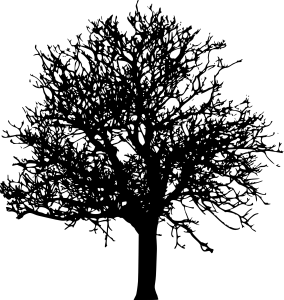
\includegraphics[width=2.08333in,height=\textheight,keepaspectratio]{tree_01.png}

}

\caption{\label{fig-arbol01}Árbol}

\end{figure}%

Algunos ejemplos de inclusión de etiquetas:

\begin{itemize}
\item
  \texttt{!{[}Árbol{]}(tree\_01.png)\{\#fig-arbol01\ width=200\}} y
  luego se puede \textbf{citar} usando el símbolo \texttt{@} seguido de
  la etiqueta completa del elemento que nos interesa citar:

  \begin{itemize}
  \tightlist
  \item
    Vea \texttt{@fig-arbol01} como ilustración: Vea
    Figura~\ref{fig-arbol01} como ilustración
  \item
    \texttt{@Fig-arbol01}: Figura~\ref{fig-arbol01}
  \item
    \texttt{{[}Fig.\ @fig-arbol01{]}}: Fig.~\ref{fig-arbol01}
  \item
    \texttt{{[}-@fig-arbol01{]}}: \ref{fig-arbol01}
  \end{itemize}
\end{itemize}

Un ejemplo de definición, sería:

\begin{definition}[Línea
recta]\protect\hypertarget{def-linea}{}\label{def-linea}

La ecuación de una línea recta, llamada ecuación lineal, puede
escribirse como:

\begin{equation}\phantomsection\label{eq-linea}{
y = mx + b
}\end{equation}

\end{definition}

Véase def.~\ref{def-linea} y Ecuación~\ref{eq-linea}.

Se ha escrito:

\begin{Shaded}
\begin{Highlighting}[]
\NormalTok{::: \{\#def{-}linea\}}

\FunctionTok{\#\# Línea recta}

\NormalTok{La ecuación de una línea recta, llamada ecuación lineal, puede escribirse como:}

\NormalTok{$$}
\NormalTok{y = mx + b}
\NormalTok{$$ \{\#eq{-}linea\}}
\NormalTok{:::}

\NormalTok{Véase }\CommentTok{[}\OtherTok{def. @def{-}linea}\CommentTok{]}\NormalTok{ y @eq{-}linea.}
\end{Highlighting}
\end{Shaded}

Existen entornos matemáticos que no se suelen numerar:
``demostraciones'' (``proof''), ``soluciones'' (``solution''), ``notas''
(``remark''). Por ejemplo, escribir un entorno con la solución de algún
ejercicio:

\begin{solution}
La solución del ejercicio es \ldots{}
\end{solution}

Se ha escrito:

\begin{Shaded}
\begin{Highlighting}[]
\NormalTok{::: \{.solution\}}
\NormalTok{La solución del ejercicio es ...}
\NormalTok{:::}
\end{Highlighting}
\end{Shaded}

\begin{tcolorbox}[enhanced jigsaw, rightrule=.15mm, toprule=.15mm, opacitybacktitle=0.6, arc=.35mm, toptitle=1mm, left=2mm, colback=white, colbacktitle=quarto-callout-note-color!10!white, opacityback=0, colframe=quarto-callout-note-color-frame, breakable, coltitle=black, bottomtitle=1mm, titlerule=0mm, title=\textcolor{quarto-callout-note-color}{\faInfo}\hspace{0.5em}{Nota}, bottomrule=.15mm, leftrule=.75mm]

Al final del documento, \textbf{automáticamente} se muestra el apartado
correspondiente a la bibliografía o referencias bibliográficas que han
sido citadas-incluidas en este documento, formateadas.

\end{tcolorbox}


  \bibliography{local.bib}



\end{document}
